\documentclass[12pt]{standalone}
\usepackage{tikz}
%\usetikzlibrary{calc, arrows.meta, decorations.pathreplacing}

% Assume $X$ is Hausdorff, and let
% $\(a\,b\)in X times X\\Delta,$ that is $a eq.not b$ in $X.$ The
% definition of product topology tells us that to show that
% $X times X\\Delta$ is open, we need to find an open rectangle $R_(a\,b)$
% such that $\(a\,b\)in R_(a\,b) subset.eq X times X\\Delta.$
%  
% By definition of 'Hausdorff', there exists disjoint open sets
% $U in.rev a$ and $V in.rev b$ in $X.$ Denote $U times V$ by $R_(a\,b).$
% Then, as required, $R_(a\,b)$ contains the point $\(a\,b\)$ and is
% contained in $X times X\\Delta,$ because $U inter V = nothing$ means
% that $U times V$ cannot contain points of the form $\(x\,x\).$
% We have proved that $X times X\\Delta$ is open, so $Delta$ is closed in $X times X.$

\usetikzlibrary{arrows.meta, patterns}
\begin{document}

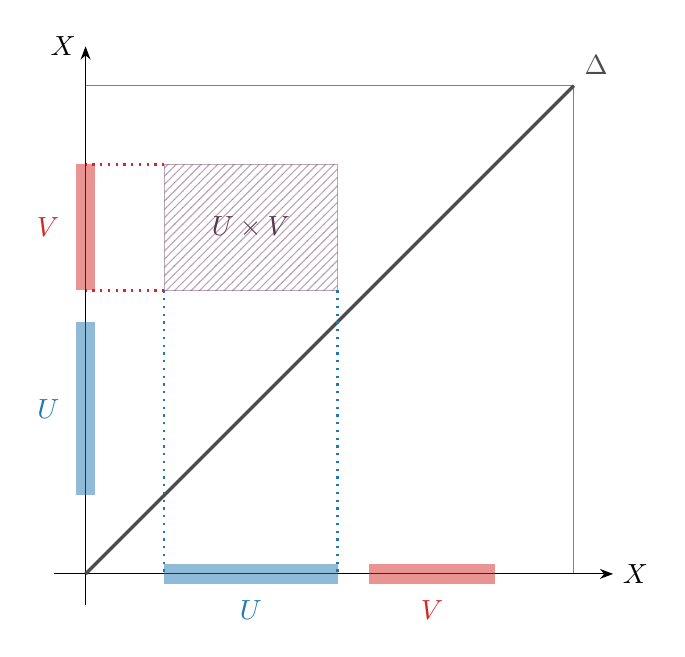
\begin{tikzpicture}[>=Stealth, scale=1]

  % ---- parameters: U = (ua,ub), V = (va,vb), with ub < va ----
  \def\ua{1.0}\def\ub{3.2}
  \def\va{3.6}\def\vb{5.2}

  % ---- colours ----
  \definecolor{Ucol}{RGB}{31,119,180}   % blue
  \definecolor{Vcol}{RGB}{214,39,40}    % red
  \colorlet{UVcol}{Ucol!50!Vcol}

  % ---- the space X x X ----
  \draw[gray] (0,0) rectangle (6.2,6.2);

  % ---- axes ----
  \draw[->] (-0.4,0) -- (6.7,0) node[right] {$X$};
  \draw[->] (0,-0.4) -- (0,6.7) node[left] {$X$};

  % ---- diagonal ----
  \draw[very thick, black!70] (0,0) -- (6.2,6.2)
        node[above right] {$\Delta$}; % =\{(x,x): x\in X\}$};

  % ---- the open rectangle U x V (dashed boundary, since it is open) ----
 %  \fill[UVcol!30] (\ua,\va) rectangle (\ub,\vb);
 %  \draw[dashed, thick, UVcol!80!black] (\ua,\va) rectangle (\ub,\vb);
 \filldraw[UVcol, pattern color=UVcol, pattern=north east lines, opacity=0.5] (\ua,\va) rectangle (\ub,\vb);
  \node[UVcol!70!black] at ({(\ua+\ub)/2},{(\va+\vb)/2}) {$U\times V$};

  % ---- dotted projection lines from the rectangle to the axes ----
  \draw[dotted, thick, Ucol] (\ua,\va) -- (\ua,0);
  \draw[dotted, thick, Ucol] (\ub,\va) -- (\ub,0);
  \draw[dotted, thick, Vcol] (\ua,\va) -- (0,\va);
  \draw[dotted, thick, Vcol] (\ua,\vb) -- (0,\vb);

  % ---- faint guides: where U and V sit on the "other" axes ----
  %\draw[dotted, Ucol!50] (0,\ua) -- (\ua,\ua);
  %\draw[dotted, Ucol!50] (0,\ub) -- (\ub,\ub);
  %\draw[dotted, Vcol!50] (\va,0) -- (\va,\va);
  %\draw[dotted, Vcol!50] (\vb,0) -- (\vb,\vb);

  % ---- intervals on the horizontal axis ----
  \draw[line width=7pt, opacity=0.5, Ucol] (\ua,0) -- (\ub,0);
  \draw[line width=7pt, opacity=0.5, Vcol] (\va,0) -- (\vb,0);

  % ---- intervals on the vertical axis ----
  \draw[line width=7pt, opacity=0.5, Ucol] (0,\ua) -- (0,\ub);
  \draw[line width=7pt, opacity=0.5, Vcol] (0,\va) -- (0,\vb);

  % ---- open endpoints (hollow circles) ----
%  \foreach \p in {\ua,\ub} {
%    \draw[Ucol, fill=white, thick] (\p,0) circle (2.5pt);
%    \draw[Ucol, fill=white, thick] (0,\p) circle (2.5pt);
 % }
 % \foreach \p in {\va,\vb} {
 %   \draw[Vcol, fill=white, thick] (\p,0) circle (2.5pt);
 %   \draw[Vcol, fill=white, thick] (0,\p) circle (2.5pt);
 % }

  % ---- labels for the intervals ----
  \node[Ucol, below=6pt] at ({(\ua+\ub)/2},0) {$U$};
  \node[Vcol, below=6pt] at ({(\va+\vb)/2},0) {$V$};
  \node[Ucol, left=6pt]  at (0,{(\ua+\ub)/2}) {$U$};
  \node[Vcol, left=6pt]  at (0,{(\va+\vb)/2}) {$V$};

\end{tikzpicture}

\end{document}
